\begin{figure}
\centering

\ifpdf
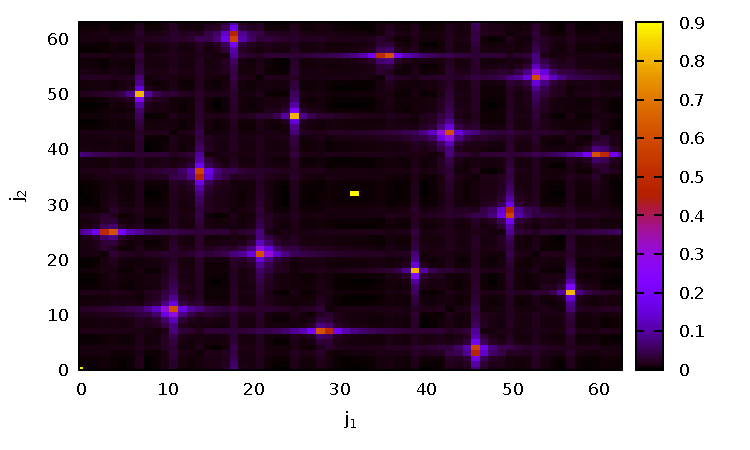
\includegraphics[angle=0]
{./part4/quantcomp/picdiscretlog3.pdf}
\else
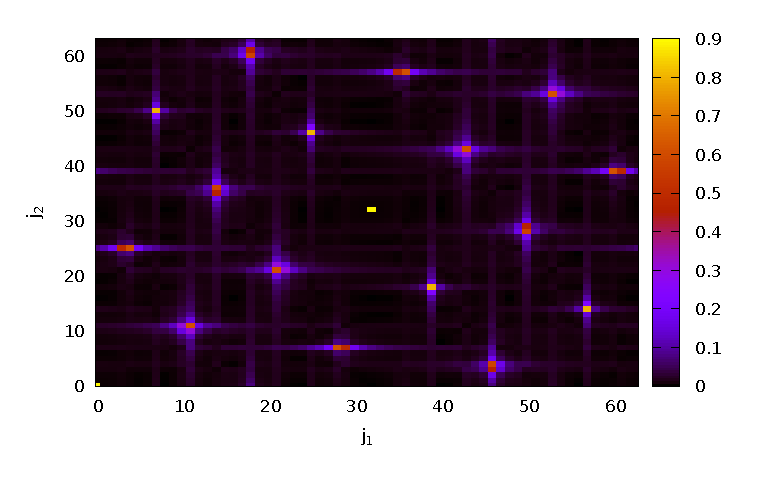
\includegraphics[angle=0]
{./part4/quantcomp/picdiscretlog3.eps}
\fi

%\input ./part4/quantcomp/picdiscretlog2.tex

\caption{Fourier transform of the samples of the function 
$f'(x_1, x_2)$
Number of samples $M=64$. Coordinates of the maximum $j_1 \approx 46$, $j_2 \approx 3.5$. 
The solution of the equation $3^x \equiv 14 \mod 19$
is $x = 13 \approx \frac{46}{3.5} \approx 13.14$
} 
\label{fig:part4:quantcomp:dl3}
\end{figure}